% Complete Section 4.2, original PDF 45-47 / printed 35-37.
% mathsf H is the non-Fraktur harmonic space; mathcal H remains cohomology.
% block: harmonic-hodge-poincare-heading page:45 type:section
\subsection{{调和形式, Hodge 分解与 Poincaré 不等式}}\label{sec:harmonic-hodge-poincare}

% block: hilbert-structure-consequences page:45 type:ordinary-paragraph
{接下来推导 Hilbert 空间结构的几个简单而关键的推论. 本节假设 $(W,d)$ 是 Hilbert 复形, 不一定是闭的.}

% block: harmonic-forms-heading page:45 type:subsection
\subsubsection{{调和形式}}\label{subsec:harmonic-forms}

% block: harmonic-form-definition page:45 type:definition
\Needspace{6\baselineskip}
\begin{Definition}\label{def:harmonic-form}
{若元素 $v\in W^k$ 同时满足 $dv=0$ 和 $d^*v=0$, 则称其为\emph{调和的}, 或称为\emph{调和 $k$-形式}.}
\end{Definition}

% block: harmonic-space-definition page:45 type:ordinary-paragraph
{将调和 $k$-形式的空间记为 $\mathsf H^k$, 因此 $\mathsf H^k=\mathcal Z^k\cap\mathcal Z_k^*$. 由 Theorem~\ref{thm:adjoint-kernel-range-orthogonality} 的第一个断言, 也可以写成}
\begin{equation}\label{eq:harmonic-cocycle-orthogonality}
\mathsf H^k=\mathcal Z^k\cap\mathcal B^{k,\perp},
\end{equation}

% block: harmonic-reduced-cohomology page:45 type:ordinary-paragraph
{其含义是, 调和形式就是与上边界链正交的闭上链. 若上边界链空间不闭, 可取其闭包, 并等价地说, $\mathsf H^k$ 是闭子空间 $\overline{\mathcal B}^k$ 在 Hilbert 空间 $\mathcal Z^k$ 中的正交补. 因而可以典范地将商空间, 即约化上同调空间 $\mathcal Z^k/\overline{\mathcal B}^k$, 与 $W^k$ 的子空间 $\mathsf H^k$ 等同. 当然, 对闭 Hilbert 复形, 无须特别指明约化, 结论就是}
\begin{equation}\label{eq:harmonic-cohomology-isomorphism}
\mathsf H^k\cong\mathcal H^k.
\end{equation}

% block: harmonic-canonical-representatives pages:45,46 type:ordinary-paragraph
{因此, 调和形式将复形的上同调具体实现为 Hilbert 空间 $W^k$ 的一个闭子空间. Figure~\ref{fig:cohomology-harmonic-representatives} 展示了这一点. 上同调空间 $\mathcal H^k$ 的元素是 $\mathcal Z^k$ 的元素模 $\mathcal B^k$ 的等价类. 这些等价类将 $\mathcal Z^k$ 分解为由 $\mathcal B^k$ 平移得到的闭仿射子空间. 每个这样的子空间都含有一个特殊元素, 即唯一与 $\mathcal B^k$ 正交的元素, 它也可刻画为唯一的最小范数元素. 这些就是调和 $k$-形式.}

% block: cohomology-geometry-figure page:45 type:figure
\begin{figure}[htbp]\centering
% Native-vector transcription of original Figure 4.1, PDF 45 / printed 35.
% Non-Fraktur label mapping is explicit in config/math-alphabet-policy.json.
% Preserve the plane, parallel affine lines, orthogonal harmonic line, 0, z_0, z and [z].
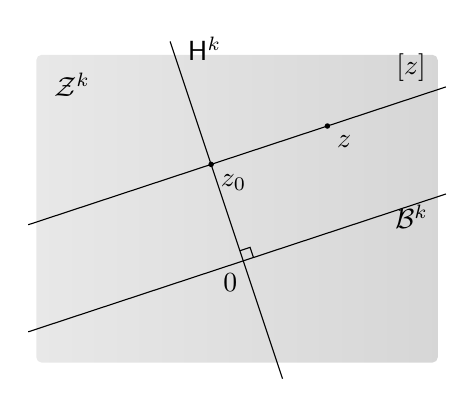
\begin{tikzpicture}[x=.85cm,y=.85cm]
\shade[rounded corners=2pt,left color=gray!18,right color=gray!32] (0,0) rectangle (6,4.6);
\draw (-.12,.4604)--(6.12,2.5196);
\draw (-.12,2.0604)--(6.12,4.1196);
\draw (2,4.8)--(3.68,-.24);
\coordinate (origin) at (3.0931,1.5207);
\coordinate (representative) at (2.6126,2.9622);
\coordinate (cycle) at (4.35,3.5355);
\draw (origin) ++(.1519,.0501)--++(-.0501,.1519)--++(-.1519,-.0501);
\fill (representative) circle (1pt);
\fill (cycle) circle (1pt);
\node[anchor=north east] at (3.15,1.48) {$0$};
\node[anchor=north west] at (representative) {$z_0$};
\node[anchor=north west] at (cycle) {$z$};
\node[anchor=south] at (5.6,4.05) {$[z]$};
\node[anchor=north west] at (.12,4.48) {$\mathcal Z^k$};
\node[anchor=south west] at (2.12,4.37) {$\mathsf H^k$};
\node[anchor=north east] at (6,2.5) {$\mathcal B^k$};
\end{tikzpicture}

\caption{{上边界链空间 $\mathcal B^k$ 是闭上链空间 $\mathcal Z^k$ 的子空间. 上同调空间由闭上链的等价类组成, 其中闭上链 $z$ 的类 $[z]$ 是经过 $z$ 且平行于 $\mathcal B^k$ 的仿射子空间. 每个上同调类 $[z]$ 由属于 $\mathsf H^k$ 的唯一元素 $z_0$ 表示, 它是该类中范数最小的元素.}}\label{fig:cohomology-harmonic-representatives}
\end{figure}

% block: compactness-property-intro page:46 type:ordinary-paragraph
{可利用调和形式得到 Hilbert 复形为 Fredholm 的一个有用判据, 即其同调空间为有限的判据. 空间 $V^k\cap V_k^*\subset W^k$ 配备下述范数后是 Hilbert 空间:}
\[
\|v\|_{V\cap V^*}^2=\|v\|_V^2+\|v\|_{V^*}^2=2\|v\|^2+\|dv\|^2+\|d^*v\|^2.
\]

% block: hilbert-norm-conventions page:46 type:ordinary-paragraph
{这里及下文, 用 $\|\cdot\|_V$ 表示各空间 $V^k$ 中的范数, 用 $\|\cdot\|_{V^*}$ 表示空间 $V_k^*$ 中的范数, 并简单地用 $\|\cdot\|$ 表示空间 $W^k$ 中的范数.}

% block: compactness-property-definition page:46 type:definition
\Needspace{6\baselineskip}
\begin{Definition}\label{def:hilbert-complex-compactness-property}
{若对每个 $k$, 包含映射 $V^k\cap V_k^*\subset W^k$ 都是紧的, 则称 Hilbert 复形具有紧性性质.}
\end{Definition}

% block: compactness-implies-fredholm page:46 type:theorem
\Needspace{6\baselineskip}
\begin{Theorem}\label{thm:compactness-implies-fredholm}
{若 Hilbert 复形具有紧性性质, 则它是闭的且为 Fredholm 复形.}
\end{Theorem}

% block: compactness-closed-range-proof page:46 type:proof
\begin{Proof}
{先验证 $d$ 的像空间是闭的. 设 $T$ 为 $d$ 在 $D(T):=V\cap\mathcal Z^\perp$ 上的限制, 视为无界算子 $W\to W$. 容易验证 $T$ 的像空间与 $d$ 的像空间相同, 且由于 $d$ 是闭算子, $T$ 也闭. 由于 $\mathcal Z^\perp=\overline{\mathcal B}^*\subset\mathcal Z^*\subset V^*$, 有 $D(T)\subset V\cap V^*$, 且 $D(T)$ 上的图范数与 $V\cap V^*$ 范数等价. 由 Theorem~\ref{thm:compact-domain-closed-range}, $T$ 从而 $d$ 均有闭像空间.}

% block: compactness-finite-dimensional-proof page:46 type:proof
{其次注意, 在 $\mathsf H\subset V\cap V^*$ 上, $V\cap V^*$ 范数与 $W$ 范数等价. 因此 $\mathsf H$ 中的闭单位球是紧的, 这意味着 $\mathsf H\cong\mathcal H$ 为有限维, 即该复形是 Fredholm 的.}
\end{Proof}

% block: hodge-decomposition-heading page:46 type:subsection
\subsubsection{{Hodge 分解}}\label{subsec:hodge-decomposition}

% block: hodge-helmholtz-intro page:46 type:ordinary-paragraph
{Hilbert 复形结构直接导出 Hodge 分解, 它是向量微积分中 Helmholtz 分解的推广.}

% block: cocycle-orthogonal-decomposition page:46 type:ordinary-paragraph
{由于调和 $k$-形式的空间是 $\overline{\mathcal B}^k$ 在 $\mathcal Z^k$ 中的正交补, 立即有}
\begin{equation}\label{eq:cocycle-harmonic-decomposition}
\mathcal Z^k=\overline{\mathcal B}^k\BookOrthSum\mathsf H^k,
\end{equation}

% block: orthogonal-sum-definition page:46 type:ordinary-paragraph
{其中符号 $\BookOrthSum$ 表示正交的和 (注意, 在这一背景下, 无须区分 $W$ 中的正交与 $V$ 中的正交). 由于 $\mathcal Z^k$ 同时是 $W^k$ 和 $V^k$ 的闭子空间, 有}
\[
W^k=\mathcal Z^k\BookOrthSum\mathcal Z^{k\perp}=\mathcal Z^k\BookOrthSum\overline{\mathcal B}_k^*,\qquad V^k=\mathcal Z^k\BookOrthSum\mathcal Z^{k\perp V},
\]
{其中 $\mathcal Z^{k\perp V}=\mathcal Z^{k\perp}\cap V=\overline{\mathcal B}_k^*\cap V$. 结合 \eqref{eq:cocycle-harmonic-decomposition} 得到 Hodge 分解.}

% block: hodge-decomposition-theorem page:47 type:theorem
\Needspace{8\baselineskip}
\begin{Theorem}{Hodge {分解}}\label{thm:hodge-decomposition}
{任意 Hilbert 复形均给出正交分解}
\begin{equation}\label{eq:hodge-base-decomposition}
\begin{tikzpicture}[baseline=(m.base)]
\matrix (m) [matrix of math nodes,ampersand replacement=\&,column sep=6pt,inner sep=0pt] {
W^k={}\&\overline{\mathcal B}^k\&\BookOrthSum\&\mathsf H^k\&\BookOrthSum\&\overline{\mathcal B}_k^*\\};
\draw[decorate,decoration={brace,amplitude=4pt}] ([yshift=6pt]m-1-2.north west)--([yshift=6pt]m-1-4.north east) node[midway,above=5pt] {$\mathcal Z^k=\mathcal B_k^{*\perp}$};
\draw[decorate,decoration={brace,amplitude=4pt}] ([yshift=6pt]m-1-6.north west)--([yshift=6pt]m-1-6.north east) node[midway,above=5pt] {$\mathcal Z^{k\perp}$};
\draw[decorate,decoration={brace,mirror,amplitude=4pt}] ([yshift=-6pt]m-1-2.south west)--([yshift=-6pt]m-1-2.south east) node[midway,below=5pt] {$\mathcal Z_k^{*\perp}$};
\draw[decorate,decoration={brace,mirror,amplitude=4pt}] ([yshift=-6pt]m-1-4.south west)--([yshift=-6pt]m-1-6.south east) node[midway,below=5pt] {$\mathcal Z_k^*=\mathcal B^{k\perp}$};
\end{tikzpicture}
\end{equation}
{以及}
\begin{equation}\label{eq:hodge-domain-decomposition}
V^k=\overline{\mathcal B}^k\BookOrthSum\mathsf H^k\BookOrthSum\mathcal Z^{k\perp V}.
\end{equation}
\end{Theorem}

% block: hodge-closed-complex-description page:47 type:ordinary-paragraph
{对闭 Hilbert 复形, 当然可以去掉边界链空间上的横线. 此时, Hodge 分解说明 $W$ 的每个元素都唯一地分解为 $d$ 的像中的一个元素, $d^*$ 的像中的一个元素以及一个调和形式, 且该分解是正交的.}

% block: poincare-subheading page:47 type:subsection
\subsubsection{Poincaré {不等式}}\label{subsec:hilbert-poincare-inequality}

% block: poincare-intro page:47 type:ordinary-paragraph
{最后推导的结论是 Poincaré 不等式, 为此必须假设 Hilbert 复形是闭的.}

% block: hilbert-poincare-inequality page:47 type:theorem
\Needspace{6\baselineskip}
\begin{Theorem}{Poincaré {不等式}}\label{thm:hilbert-complex-poincare}
{给定闭 Hilbert 复形, 对每个 $k$, 存在常数 $c_P$, 使得}
\begin{equation}\label{eq:hilbert-poincare-inequality}
\|z\|_V\leq c_P\|dz\|,\qquad z\in\mathcal Z^{k\perp V}.
\end{equation}
\end{Theorem}

% block: hilbert-poincare-proof page:47 type:proof
\begin{Proof}
{由于 Hilbert 复形是闭的, $\mathcal B^{k+1}$ 是 Hilbert 空间. 因而算子 $d^k$ 是 Hilbert 空间 $\mathcal Z^{k\perp V}$ 与 $\mathcal B^{k+1}$ 之间的有界线性同构, 所以它具有有界逆, 由此直接得到 \eqref{eq:hilbert-poincare-inequality}.}
\end{Proof}
